% !TeX root = ../main.tex
% Add the above to each chapter to make compiling the PDF easier in some editors.

\chapter{Background}\label{chapter:background}

% Start from volume rendering, real time rendering, History, Gaussian Splatting, training process, the whole overview of the system, Results, limitations, then focus on depth extraction, blender, synthetic data, transfer functions

\section{Linear Transformation Techniques}

Linear transformation \parencite{linear-trans}, or often also called a linear mapping or linear function, is a transformation of vectors from one vector space to the other \((T: V \rightarrow W\)). Linear transformations between vectors can be represented by matrices.

\subsection{Translation}

Translation \parencite{linear-operation} is a type of geometric transformation where a point in a coordinate system is moved a certain distance in a certain direction. It can be interpreted as a simple addition operation. Given a translation vector \(\Vec{v}\) and an initial point \(p\), the translation function \(T_{\Vec{v}}\) is as follows:

\begin{center}
    \(T_{\Vec{v}}(p) = p + \Vec{v}\) 
\end{center}

\subsection{Rotation}

Rotation is another type of geometric transformation where a point is rotated against a certain reference. A standard rotation in a two-dimensional (2D) space can be described as follows:

\begin{center}
    \(R(\theta) = 
    \begin{bmatrix}
        cos\theta & -sin\theta \\
        sin\theta & cos\theta
    \end{bmatrix}
    \),
\end{center}
with \(\theta\) representing the angle of the rotation.

In the three-dimensional (3D) plane, rotations about the \(x-, y-,\) and \(z-\)planes can be described as follows:

\begin{center}
    \(R_x(\theta) = 
    \begin{bmatrix}
        1 & 0 & 0 \\
        0 & cos\theta & -sin\theta \\
        0 & sin\theta & cos\theta
    \end{bmatrix}
    \)

    \(R_y(\theta) =
    \begin{bmatrix}
        cos\theta & 0 & sin\theta \\
        0 & 1 & 0 \\
        -sin\theta & 0 & cos\theta
    \end{bmatrix}
    \)

    \(R_z(\theta) =
    \begin{bmatrix}
        cos\theta & -sin\theta & 0 \\
        sin\theta & cos\theta & 0 \\
        0 & 0 & 1
    \end{bmatrix}
    \)
\end{center}

\section{Novel View Synthesis}

Novel view synthesis (NVS) is a branch of research that focuses on the reconstruction of 3D scenes from a limited number of input images that normally represent a limited amount of differing viewpoints of the scene. The main task being tackled here is to be able to construct the scene from all other angles that are previously not provided by the input images \parencite{SynSin}. 

\subsection{Motion Parallax and Depth Extraction}

\begin{figure}[h]
    \centering
    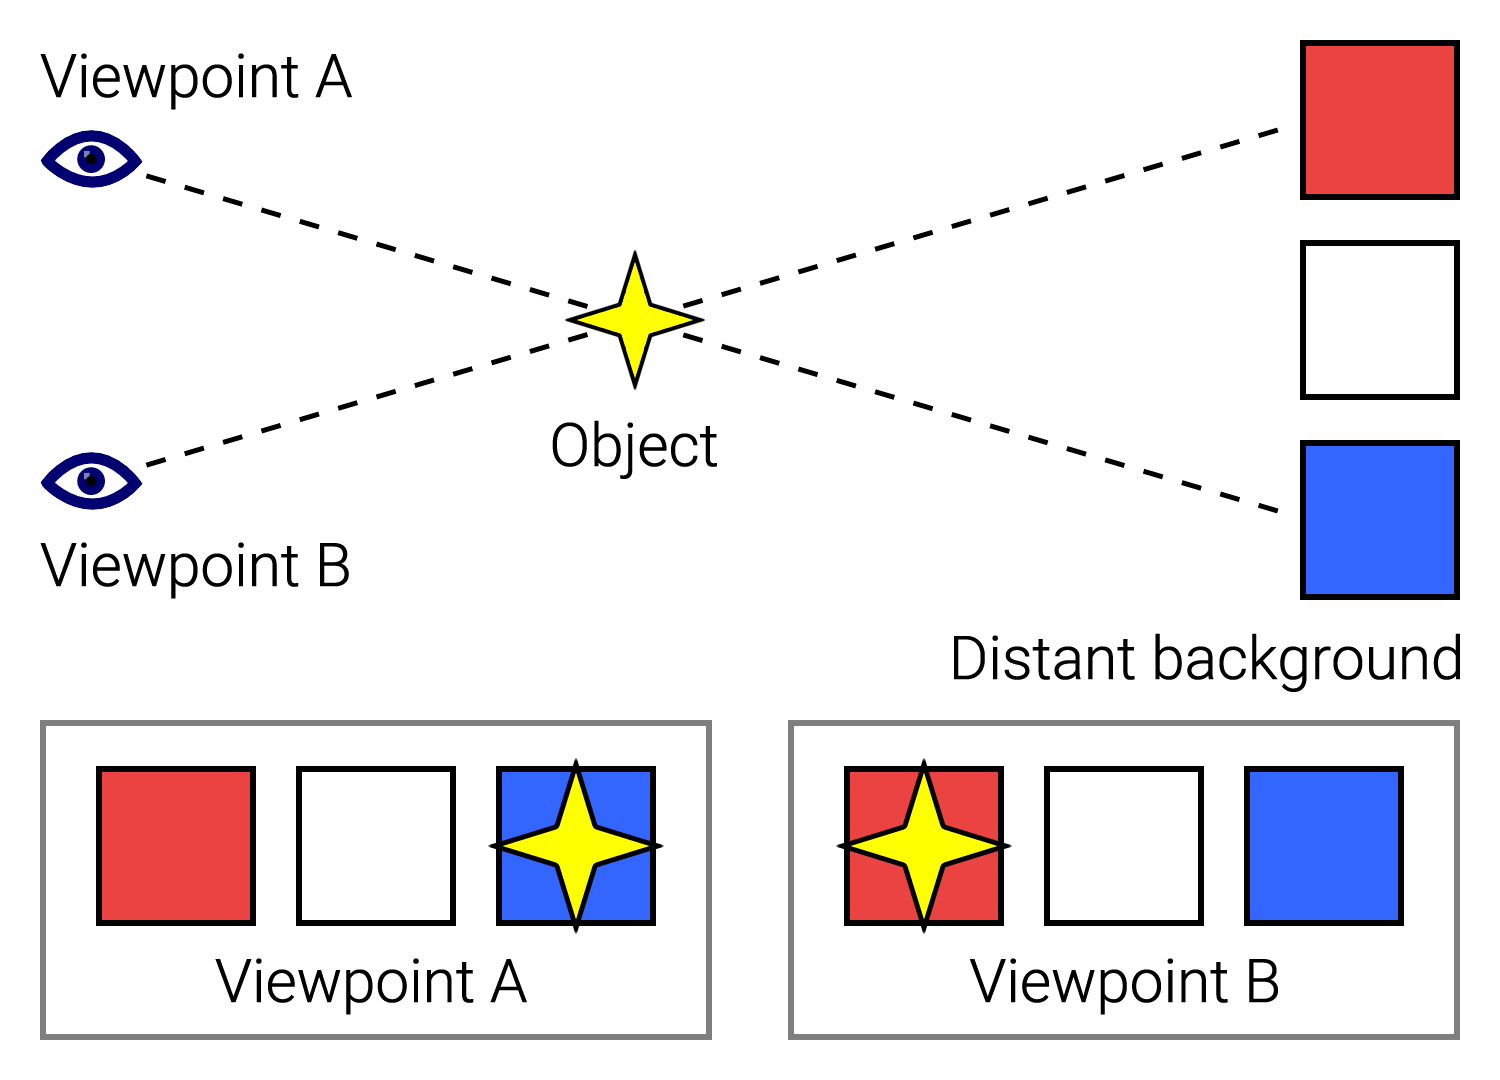
\includegraphics[width=0.5\linewidth]{figures/parallax_example_01.png}
    \caption{Parallax effect when viewing an object from two different viewpoints}
    \label{fig:parallax_01}
\end{figure}

Throughout its early development stages, one key idea mainly used to handle NVS problems is to take advantage of motion parallax: when an observer (usually denoted as the camera) moves around a scene, objects will naturally "move" from the current point of view depending on their distances from this observer \parencite{cvbook2001}. Parallax is defined as the visual phenomenon where displacement or difference in the position of an object seem to change when viewed from different points of view \parencite{CambridgeParallax}. Objects that are located closer to the observer will display a larger parallax effect when compared to objects that are farther away. Distance of the object can, due to this, be measured by measuring angles and observing the parallax. This distance can then be interpreted as depth value from the observer's point of view.

\subsection{Distance Measurement}

Distance measurement using parallax distance is based on the principle of triangulation. Triangulation is a technique developed to determine the location of a point in 3D space by forming triangles to this point from other points that are already known.

\begin{figure}[h]
    \centering
    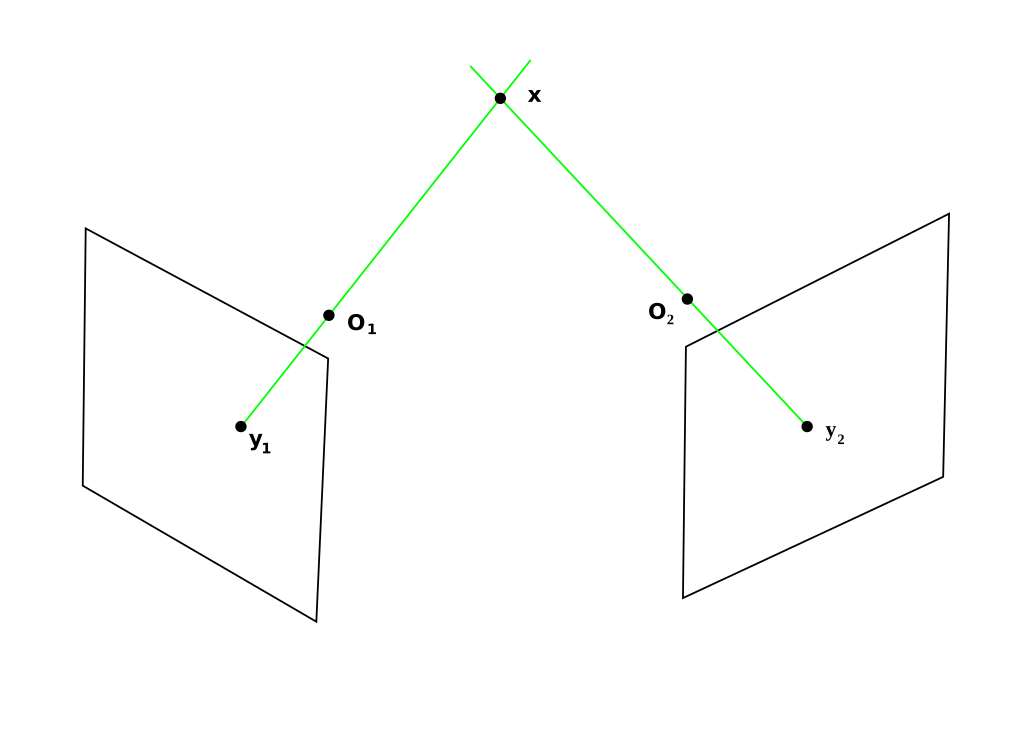
\includegraphics[width=0.5\linewidth]{figures/triangulation_example_01.png}
    \caption{3D point projection onto two different 2D images}
    \label{fig:triangulation-1}
\end{figure}

Given two different 2D images of a scene with known camera parameters, if we want to know where a certain point of an object is located on a 3D plane, we can first extract the 2D coordinates (image points) of the same point from the two different images. Since we are also given each camera's parameters, we are also able to determine the focal point of both cameras in 3D space. Consequently, we are able to draw two different lines from each image points to their respective focal points in 3D space (or from the center or location of the camera in 3D space towards the image point). These two lines will, eventually and inevitably, intersect at a point in 3D space: this point can then be regarded as the location of our point in the 3D space. Next, to determine the exact distance, we first obtain the angle created by this intersection and use this along with the disparity between the two images (distance between the two camera centers) to calculate the depth, which is the height of the triangle (see Figure \ref{fig:triangulation-2}) \parencite{triangulation}:

\begin{center}
    \(d = \frac{0.5 \cdot b}{tan(0.5 \cdot \alpha)}\),
\end{center}
with \(d\) as the distance value we are trying to find, \(b\) as the distance between two camera centerpoints, and \(\alpha\) as the angle created by the intersection.

\begin{figure}[h]
    \centering
    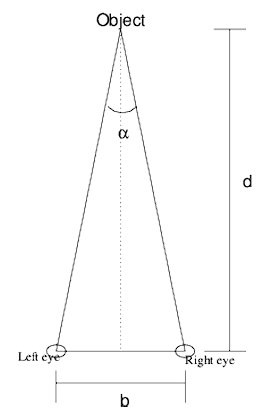
\includegraphics[height=0.5\linewidth]{figures/triangulation_example_02.png}
    \caption{distance measurement principle from triangulation technique}
    \label{fig:triangulation-2}
\end{figure}

\subsection{Structure from Motion}

\begin{figure}[h]
    \centering
    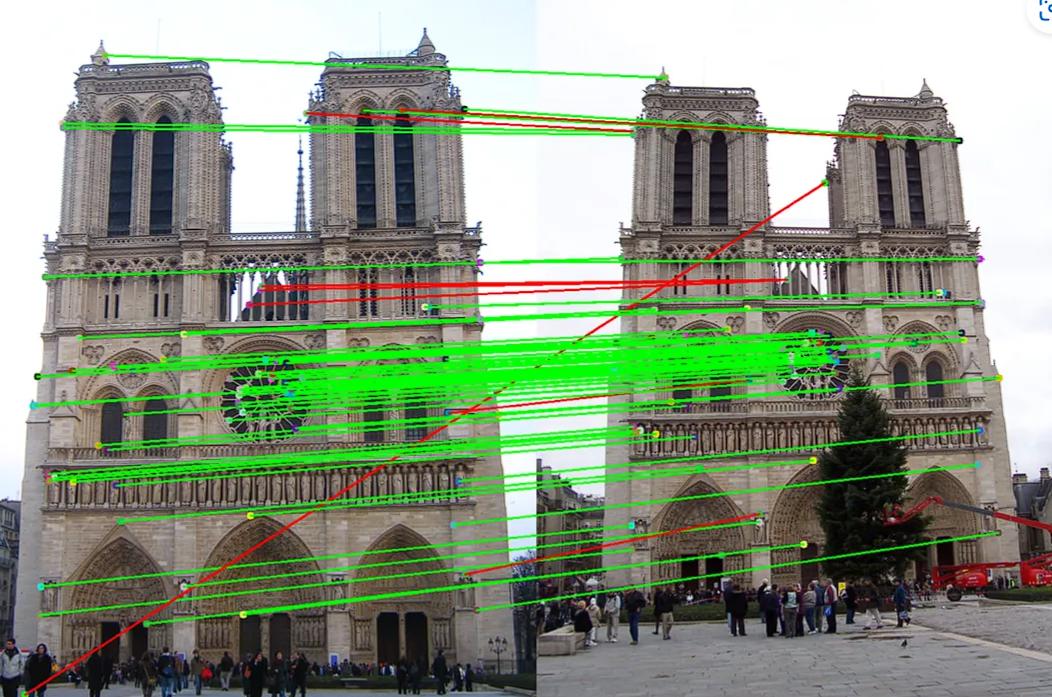
\includegraphics[height=0.5\linewidth]{figures/feature-matching.png}
    \caption{example of feature matching step}
    \label{fig:feature-matching}
\end{figure}

Following this main idea, various Structure from Motion (SfM) techniques are then developed to be able to specifically calculate points in a 3D plane purely based on 2D transformations of the projected images \parencite{sfm-base}. SfM techniques generally follow the same basic steps. Firstly, we try to find points from different points of view that correspondent to each other. This step is called feature extraction and feature matching. Typically, this is done by identifying some distinct "key points" in each image. These points are normally corners of an object. A minimum of 8 points are required, hence why this method is known as the Eight-point algorithm \parencite{8pointalg}. After these points are identified, they are then matched to the other key points from all other images and then compared (see Figure \ref{fig:feature-matching}).

\begin{figure}[h]
    \centering
    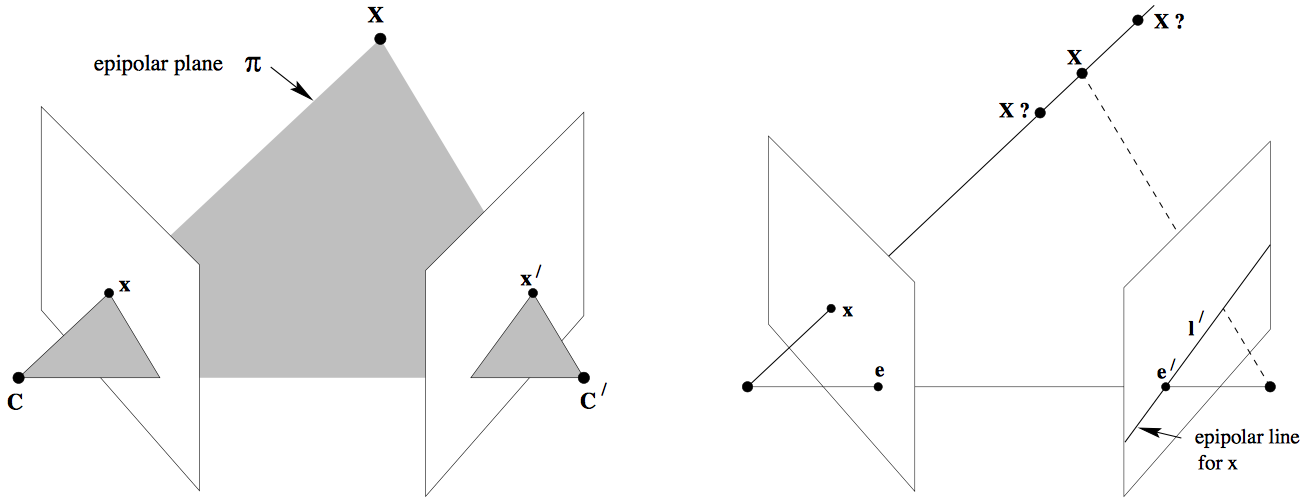
\includegraphics[width=0.5\linewidth]{figures/epipolar_geometry_01.png}
    \caption{epipolar geometry}
    \label{fig:epipolar}
\end{figure}

Next, epipolar geometry is used to relate the points previously matched with the cameras. Given a single point in 3D-space \(\mathbf{X}\) which is captured as \(\mathbf{x}\) and \(\mathbf{x}'\) in two different images, we are able to relate these two points with their respective camera centers \(\mathbf{C}\) and \(\mathbf{C}'\). Since the three points (the original point and the two projected points) are coplanar, which means they lie in the same plane \parencite{coplanar}, we can create a relationship between them as follows:

\begin{center}
    \(\Vec{\mathbf{Cx}} \cdot (\Vec{\mathbf{CC'}} \times \Vec{\mathbf{C'x'}}) = 0\)
\end{center}

As for the rest, it is only a matter of applying triangulation strategies as aforementioned to get the desired points in space.

For the final step, bundle adjustment \parencite{bundle-adj} is done to refine the 3D points gained from the previous calculations to minimize the cost function and filter out unneeded 3D points. This is done by minimizing the reprojection error, which is essentially a geometric error that pertains to the distance between an estimated point and the actual projected point \parencite{epipolar}.

\section{Monocular Depth Estimation}

Monocular Depth Estimation (MDE) is a classical task in the computer vision field, commonly regarded as a problem under simultaneous localization and mapping (SLAM) \parencite{slam-ex}, with a very broad usage in critical fields such as navigation \parencite{mde-navigation} and object detection \parencite{mde-obstacle}. Given a single monocular RGB image, this problem focuses on estimating the depth values in the image.

Traditional MDE methods employ methods such as SfM and stereo calibration. More recent advancements employ the usage of neural networks and learning techniques \parencite{mde-nn-1} \parencite{dinov2} \parencite{mde-nn-2} \parencite{mde-nn-3} in order to provide a high quality output. Some notable works in this field include: 1) MiDAS \parencite{Midas}, which introduces tools to train models on different datasets, 2) ZoeDepth \parencite{ZoeDepth}, which focuses on combining Relative Depth Estimation techniques with Metric Depth Estimation techniques, and 3) Depth Anything \parencite{DepthAnythingV1} \parencite{DepthAnythingV2}, which focuses on developing a more generalist model to predict images under any scenarios.    

\section{Radiance Field Methods}

Following the advancements in SfM methods and deep learning, the neural radiance field method is discovered. Neural radiance field (NeRF) \parencite{nerf} is a deep learning technique aimed to address the task of three-dimensional (3D) reconstruction based solely on two-dimensional (2D) photographs or images of a scene. The basic NeRF algorithm outputs a scene reconstruction as a radiance field created by parameters assigned through a learning process by a deep neural network.

\subsection{NeRF Method}

\begin{figure}[h]
    \centering
    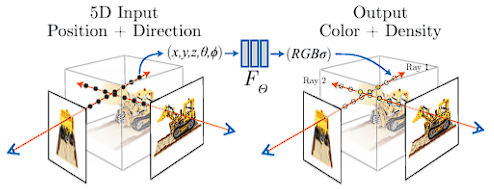
\includegraphics[]{figures/nerf-pipeline-1.png}
    \caption{illustration of the input-output scheme of NeRF \parencite{nerf}}
    \label{fig:nerf-pipeline}
\end{figure}

As input, the algorithm accepts a collection of images that represent a 3D scene from multiple viewing angles and camera poses. Each input image contains data on the image's camera's viewing direction \(d = (\theta, \phi)\), as well as the image data itself that contains information on spatial location \((x, y, z)\) in the coordinate system. Since multiple input images are received, this can then be condensed into a continuous 5D function and fed into a multilayer perceptron (MLP) network. An MLP network itself is basically a feedforward neural network that obtains a set of inputs which are then fed forward to a set of layers that are tasked to adjust a set of weights to obtain the most optimal output \parencite{feedforward}. MLPs consist of neurons that are entirely connected to each other with nonlinear activation functions and are mainly used for input data that are typically more complex and not linearly separable \parencite{mlp}. This MLP network can be represented as such (see Figure \ref{fig:nerf-pipeline}):

\begin{center}
    \(F_\Theta: (\mathbf{x, d}) \rightarrow (\mathbf{c}, \sigma)\),
\end{center}
with \(\Theta\) as the weights trained by the neural network, \(\mathbf{x}\) as our input coordinate, \(\mathbf{c}\) as the color output, and \(\sigma\) as the density output.

\subsection{Improvements to Original NeRF Method}

Since early applications of NeRF method still suffer from large optimization drawbacks, other related works aiming to improve this pipeline have since emerged. There have been some methods that optimize camera pose predictions and NeRF's volumetric function \parencite{BARF}, improve the sharpness level of details produced by the method \parencite{mipnerf}, and improved assignment of initial weights to the MLP \parencite{learned-init}. There have also been other researches that focused on improving NeRF applications for dynamic scene \parencite{nerfw} and experimentally added more outputs to enable custom lighting \parencite{relight}. Most notably, more recent methods before the introduction of Gaussian Splatting aimed to address NeRF's costly training times and pursue real-time rendering \parencite{plenoctrees} \parencite{snerg} \parencite{inerf}.

\subsection{Advantages of the NeRF Method}

One of the main advantages of NeRF method is that it is multiview consistent, which means that we are able to see representations of the reconstructed scene from different points of view and it should still be consistent and coherent. NeRF achieves this by first restricting the volume density (opacity) function to depend only on the 3D location of the point, while allowing the RGB color \(\mathbf{c}\) to be predicted based on the 3D location and the viewing direction of the camera. This ensures that the density will not change based on the viewpoint of the camera: what is dense at one point should also stay dense when looked at from other points and vice versa.

Another main advantage is that NeRF method is able to produce reconstructions of superior quality when compared to its predecessor methods. Previously, instead of outputting radiance field, the usage of deep neural networks that output discretized voxel representations are more prominent. However, when compared to these methods, NeRF was able to not only provide better reconstructions, but also maintain competitive rendering time.

\subsection{Limitations of the NeRF Method}

Despite its massive success in creating a scene reconstruction with superior quality, NeRF still suffers mainly from its long training times. While it is true that NeRF training times remain competitive when compared to other previous methods that also use deep convolutional networks, NeRF is highly restricted by hardware capabilities and compute power, since it demands a large amount of resources in exchange for quality. All advancements in NeRF methods still is restricted by the fact that it demands the usage of a full-scale neural network. Thus, it is still unable to be used for more practical applications in fields that require more real-time rendering capabilities.

\section{Gaussian Splatting} 

Gaussian Splatting is a volume rendering algorithm first introduced in 1991 by Lee Alan Westover \parencite{original-gs}. The main idea of this method is "splatting", which is the projection of volume masses directly onto the image plane during the rendering process instead of properly describing the volume as surface or line primitives and then using geometric meshes to draw the scene. The result of this algorithm delivers a point cloud -- a set of points (or, here, Gaussians) that, when rendered, represents the scene in question. 

\section{3D Gaussian Splatting}

3D Gaussian Splatting \parencite{3DGS} a major breakthrough in real-time rendering of reconstructed 3D radiance fields. It addresses NeRF's main weakness, which is its inability to render scenes in real-time. The main idea of this technique is the direct usage of "splats" of 3D Gaussians to represent scenes instead of converting data acquired from learning process into primitives first, therefore skipping an entire step in the rendering process. These 3D Gaussians retain important volumetric properties, such as density, color, and transmittance, which opens the gate for real-time rendering of high-quality multiview reconstructions of 3D scenes. Furthermore, the original 3DGS method offers further optimization on these properties in order to enhance rendered quality of the scene and also presents a faster rendering technique, runnable on GPU, that considers visibility during the rendering process and is therefore more resource-saving. 

\subsection{3DGS Pipeline}

\begin{figure}[h]
    \centering
    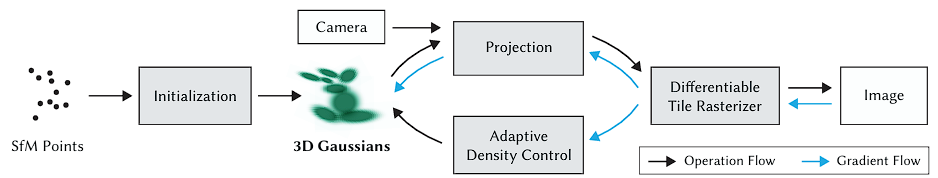
\includegraphics[width=1.0\linewidth]{figures/3dgs-optimizer-pipeline.png}
    \caption{3DGS pipeline}
    \label{fig:3dgs-optimizer-pipeline}
\end{figure}

The 3DGS method follows several important steps from start to finish. First, it accepts as input a set of 2D images, along with the corresponding camera poses and locations (and a point cloud by-product) that have been calibrated by SfM techniques (specifically, with COLMAP) \parencite{colmap1} \parencite{colmap2}. Next, the algorithm produces a set of 3D Gaussians to represent the scene. These Gaussians contain positional information, as well as covariance matrix and opacity. Afterwards, the algorithm determines the color of each pixels on the view-dependent scene using spherical harmonics \parencite{sh-1} \parencite{sh-2}. Then, a series of optimization steps are taken in order to adjust the distribution of the 3D Gaussians to ensure finer details are kept while also minimizing resource-consumption in blander areas. Lastly, a tile-based rasterizer is implemented to enable efficient and visibility-aware calculation of color. This allows fast rendering duration while also removing unnecessary resource consumption from the rendering algorithm.

\subsection{3D Gaussians}

In the traditional 3DGS method, Gaussian objects are defined as follows:

\begin{center}
    \(G(x) = e^{-\frac{1}{2}(x - x_p)^T\sum^{-1}(x - x_p)}\),
\end{center}
with \(\sum\) as a 3D covariance matrix and \(x_p\) as the center of the Gaussian \parencite{gaussian}. 

During the rendering phase, 3D Gaussians are projected onto the image space. Given viewing transformation \(W\) and Jacobian of the affine projection onto image plane \(J\), the covariance matrix \(\Sigma'\) in camera coordinates is as follows:

\begin{center}
    \(\Sigma' = J W \Sigma W^T J^T\) \parencite{gaussian}.
\end{center}
Furthermore, removing the last row and the last column from the resulting covariance matrix leaves us with the projected 2D Gaussians in the image plane.

\subsection{Alpha Blending}

For the color calculation, 3DGS method employs traditional alpha blending technique. Alpha blending is a color determination technique that considers transparency levels of different objects and also the background \parencite{alphablending}. In 3DGS, alpha blending is done from front to back as follows:

\begin{center}
    \(C = \sum\limits_{i \in N} \alpha_i c_i \prod\limits_{j = 1}^{i - 1} (1 - \alpha_j),\)
\end{center}
with \(\alpha_i\) as product of the \(i\)-th Gaussian with its opacity and \(c_i\) as the color component.

\subsection{Spherical Harmonics}

Spherical Harmonics (SH) are functions pertaining to the surface of a sphere that are often used to model different types of surfaces \parencite{sh-ex-01} \parencite{sh-ex-02}. The traditional 3DGS method closely follows SH representation of color used by NeRF methods \parencite{plenoctrees}. Rather than outputting RGB values, a function that outputs spherical harmonics coefficients is created:

\begin{center}
    \(f(x) = (\mathbf{k}, \sigma),\) with \(
    \mathbf{k} = (k^m_l)^{m:-l \leq m \leq l}_{l: 0 \leq l \leq l_{max}}.
    \)
\end{center}
Here, \(k^m_l \in \mathbb{R}^3\) represents a set of 3 coefficients corresponding to each components of RGB \parencite{plenoctrees}. With this representation, the color \(c\) at any point \(\mathbf{x}\) can be obtained with the following function:

\begin{center}
    \(c(\mathbf{d; k}) = S (\sum\limits_{l = 0}^{l_{max}} \sum\limits_{m = -l}^{l} k^m_l Y^m_l (\mathbf{d}))\),
\end{center}
with \(\mathbf{d}\) as the desired viewing angle, \(S : x \rightarrow (1 + e^{-x}))^{-1}\) as the sigmoid function for color normalization, and \(Y^m_l: \mathbb{S}^2 \rightarrow \mathbb{R}\) as the SH function in question.

\subsection{Optimization Pipeline}

The optimization step of 3DGS aims to optimize the density of the 3D Gaussians so that it would build an accurate reconstruction of the scene. In addition to this, SH coefficients from the previous step are also optimized to accurately capture the scene. This is done by doing several successive rendering iterations and comparing the rendering result to the training images (photometric loss).  

\subsection{Rasterizer Improvements for Real-Time Rendering}

The rasterization process of 3DGS is done in several steps \parencite{3DGS}. First, tile-based rasterization is performed. This step splits the screen into a \(16 \times 16\) set of tiles and then culls 3D Gaussians that do not significantly contribute to the scene representation to reduce computational overhead. Only Gaussians with a 99\% confidence interval or above are kept and Gaussians located at unreliable positions (e.g. too close or too far away) are eliminated. Next, these remaining Gaussians are sorted and alpha blending is done in a front-to-back style until full opacity is reached. Afterwards, in order to avoid excessive memory usage, the sorted list of Gaussians is traversed once again back-to-front for the backward pass step done in order to optimize the gradient computation.

\subsection{Improvements to Traditional 3DGS Method}

\begin{figure}[h]
    \centering
    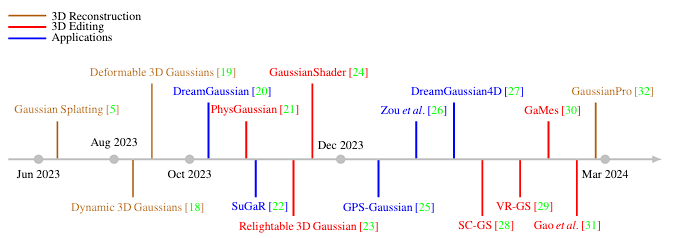
\includegraphics[width=1.0\linewidth]{figures/3dgs-timeline.png}
    \caption{A timeline depicting advancements to the 3DGS method until March 2024 \parencite{3dgs-timeline}}
    \label{fig:3dgs-timeline}
\end{figure}

Since the release of the original 3DGS method, various further iterations and improvements have been made to the method. Most notably, improvements have been made to the rendering quality of 3DGS \parencite{mipsplat} \parencite{gaussian} \parencite{gaussianpro}, explored geometric representation aspects of 3DGS \parencite{2DGS} \parencite{radegs} \parencite{gs2mesh}, or even specifically performing SLAM tasks \parencite{gs-slam} \parencite{splatam} \parencite{cg-slam}.

\subsection{Limitations of the Traditional 3DGS Method}

Since it is a newly founded technique, traditional 3DGS tend to suffer from noisy reconstructions and optimization problems. In places where the scene is not captured well, elongated artifacts may be formed. This is made even worse by the fact that antialiasing techniques have not been implemented in the original 3DGS technique. Another limitation of 3DGS is that regularization techniques are not applied during optimization. This also, in turn, contributes to the noisy reconstruction of the scenes. Furthermore, training consumes a lot of resources since the technique is still rough around the edges and sometimes, this even results in higher memory consumption when compared to NeRF models \parencite{3DGS}.
